%
%   Prof. Dr. Julian Reichwald  
%   auf Basis einer Vorlage von Prof. Dr. Jörg Baumgart
%   DHBW Mannheim 
%  
%
%	ACHTUNG: Für das Erstellen des Literaturverzeichnisses wird das modernere Paket biblatex
%			 in Kombination mit biber verwendet -- nicht mehr das ältere BibTex!  
% 			 Bitte stellen Sie ggf. Ihre TeX-Umgebung 
% 			 entsprechend ein (z.B. TeXStudio: Einstellungen --> Erzeugen --> Standard Bibliographieprogramm: biber)
%


\documentclass[
	12pt,
	BCOR=10mm,1
	headinclude=on,
	footinclude=off,
	parskip=half,
	bibliography=totoc,
	listof=entryprefix,
	toc=listof, 
	pointlessnumbers,
	plainfootsepline]{scrreprt}

%	Konfigurationsdatei einziehen
% 		HYPERREF
\usepackage[
	pdfauthor={Der Autor des Dokuments},
	pdftitle={Der Titel Ihrer Arbeit},
	hidelinks=true % keine roten Markierungen bei Links
]{hyperref}

%		FONT AND INPUT ENCODING 
%
\usepackage[T1]{fontenc}
\usepackage[utf8]{inputenc}

%
%		CALCULATIONS 
\usepackage{calc} % wird benötigt, um den kleinen Abstand nach der footsepline zu erzeugen

%		LANGUAGE SETTINGS
%
\usepackage[ngerman]{babel} 	% Voreinstellung Deutsch 
\usepackage[german=quotes]{csquotes} 	% Richtiges Setzen der Anführungszeichen mit \enquote{}  

%\usepackage[english]{babel}   %Für englische Arbeiten
%\usepackage{csquotes} 	% Richtiges Setzen der Anführungszeichen mit \enquote{}  


%		BIBLIOGRAPHY SETTINGS
%
\usepackage[backend=biber, autocite=footnote, style=authoryear-icomp, dashed=false]{biblatex} 	%Define Bibliography style 
\DefineBibliographyStrings{ngerman}{  %Change u.a. to et al. (german only!)
	andothers = {{et\,al\adddot}},             
} 
\setlength{\bibparsep}{\parskip}		%add some space between biblatex entries in the bibliography
\addbibresource{bibliography.bib}	%Add file bibliography.bib as biblatex resource 


%		GLOSSARIES AND ACRONYMS
\usepackage[printonlyused]{acronym}


%		LISTINGS
\usepackage{listings}	%Format Listings properly 
\renewcommand{\lstlistlistingname}{Quelltextverzeichnis}
\lstset{numbers=left,
	numberstyle=\tiny,
	captionpos=b,
	basicstyle=\ttfamily\small}


%		EXTRA PACKAGES 
\usepackage{lipsum}    %Blindtext
\usepackage{graphicx} %Verschiedene Grafikformate einbinden  
\usepackage[german]{varioref} 	%Bezüge etwas hübscher herstellen mit \vref
\usepackage{caption}	%bessere Captions 
\usepackage{booktabs} %schönere Tabellen


%		Algorithmen
\usepackage{algorithm}  
\usepackage{algpseudocode}
\renewcommand{\listalgorithmname}{Algorithmenverzeichnis }
\floatname{algorithm}{Algorithmus}


%		FONT SELECTION: Entweder Latin Modern oder Times / Helvetica
\usepackage{lmodern} %Latin modern font 
%\usepackage{mathptmx}  %Helvetica / Times New Roman fonts (2 lines)
%\usepackage[scaled=.92]{helvet} %Helvetica / Times New Roman fonts (2 lines)

%		PAGE HEADER / FOOTER 
%	    Achtung: In einzelnen Abschnitten der master.tex - Datei wird ggf. der innere Header redefiniert! 
\RequirePackage[automark,headsepline,footsepline]{scrpage2}
\pagestyle{scrheadings}
\renewcommand*{\pnumfont}{\upshape\sffamily}
\renewcommand*{\headfont}{\upshape\sffamily}
\renewcommand*{\footfont}{\upshape\sffamily}
\renewcommand{\chaptermarkformat}{}

\clearscrheadfoot

\ifoot[\rule{0pt}{\ht\strutbox+\dp\strutbox}DHBW Mannheim]{\rule{0pt}{\ht\strutbox+\dp\strutbox}DHBW Mannheim}
\ofoot[\rule{0pt}{\ht\strutbox+\dp\strutbox}\pagemark]{\rule{0pt}{\ht\strutbox+\dp\strutbox}\pagemark}

\ohead{\headmark}







\usepackage{setspace}

\begin{document}

\begin{titlepage}
	\begin{minipage}{\textwidth}
		\vspace{-2cm}
		\noindent \hfill   
\includegraphics{img/logo.jpg}
	\end{minipage}
	\vspace{1em}
	\sffamily
	\begin{center}
		\textsf{\large{}Duale Hochschule Baden-W\"urttemberg\\[1.5mm] Mannheim}\\[2em]
		\textsf{\textbf{\Large{}Entwicklung einer Website zur Unterstützung eines Schulsportfest}}\\[3mm]
		\textsf{\textbf{Ausarbeitung im Rahmen der Vorlesung \textit{Webprogrammierung}}} \\[1.5cm]
		\textsf{\textbf{\Large{}Studiengang Wirtschaftsinformatik}\\[3mm] \textsf{Studienrichtung Software Engineering}}
		
		\vspace{3em}
		\vfill
		
		\begin{minipage}{\textwidth}
			
			\begin{tabbing}
				Wissenschaftlicher Betreuer:\hspace{0.85cm}\=\kill
				Verfasser: \>Vincent Manz \\[1mm]
				\>Sebastian Röhling \\[1mm]
				Matrikelnummer: \> 4502972 \\[1mm]
				Kurs: \> WWI14 SE B \\[1mm]
				Studiengangsleiter: \> Prof. Dr. Thomas Holey  \\[1mm]
				Bearbeitungszeitraum: \> 19.04.2016 -- 29.06.2016
			\end{tabbing}
		\end{minipage}
		
	\end{center}
	
\end{titlepage}

\pagenumbering{roman} % Römische Seitennummerierung
\normalfont

\setstretch{1}

\chapter*{Vorwort}
Soweit im Folgenden Berufs-, Gruppen- oder Personenbezeichnungen verwendet werden, so ist stets auch die jeweils weibliche Form gemeint. Zu Gunsten des Leseflusses wird daher bewusst von einer genderneutralen Ausdrucksweise abgesehen.
\par
Um Redundanzen zu vermeiden, wurden bei manchen Stellen in der Arbeit von genaueren Erklärungen zu Quellcodeabschnitten im Text abgesehen - in diesen Fällen sind erläuternde Kommentare in den Screenshots oder in dem Code-Listing selbst vertreten.

%--------------------------------
% Verzeichnisse - nicht benötige Verzeichnisse bitte auskommentieren / löschen.
%--------------------------------

%	Inhaltsverzeichnis 
\tableofcontents

%	Abbildungsverzeichnis 
\listoffigures

%	Tabellenverzeichnis 
%\listoftables

%	Listingsverzeichnis 
\lstlistoflistings 

% 	Algorithmenverzeichnis
%\listofalgorithms

% 	Abkürzungsverzeichnis (siehe Datei acronyms.tex!)
\clearpage
\chapter*{Abkürzungsverzeichnis}	
\addcontentsline{toc}{chapter}{Abkürzungsverzeichnis}
\renewcommand*{\aclabelfont}[1]{\textbf{\textsf{\acsfont{#1}}}}


\begin{acronym}[RDBMS]
	\acro{DHBW}{Duale Hochschule Baden-Württemberg}
	\acro{RDBMS}{Relational Database Management System}
	\acro{BMBF}{Bundesministerium für Bildung und Forschung}	
\end{acronym}


%--------------------------------
% Start des Textteils der Arbeit 
%--------------------------------
\clearpage 
\ihead{\chaptername~\thechapter} % Neue Header-Definition
\pagenumbering{arabic}  % Arabische Seitenzahlen

\setstretch{1,5}
%	Einleitungs-Datei einziehen
\chapter{Einleitung}
\label{Einleitung}

\chapter{Benutzeroberfläche}
\label{Benutzeroberfläche}

\section{HTML zur Erstellung der Website}
\label{HTML zur Erstellung der Website}

\subsection{HTML-Formular Auswertung anhand einer Registrierung}
\label{HTML-Formular}

\section{CSS - Bootstrap}
\label{CSS - Bootstrap}

\subsection{Komaptibelität mit mobilen Endgeräten}
\label{Komaptibelität mit mobilen Endgeräten}

\section{Clientseitiges Javascript für benutzerspezifische Seiteninhalte}
\label{Clientseitiges Javascript}

\section{Anfahrtsbeschreibung per Google Maps}
\label{Anfahrtsbeschreibung per Google Maps}
Für den Fall, dass der Nutzer der Website von außerhalb des Ortes der Schule kommt, wurde eine Anfahrtbeschreibung mittels Google Maps eingebunden (siehe \vref{fig:googleMaps}).

\begin{figure}[!htbp]
	\makebox[\textwidth]{ 
		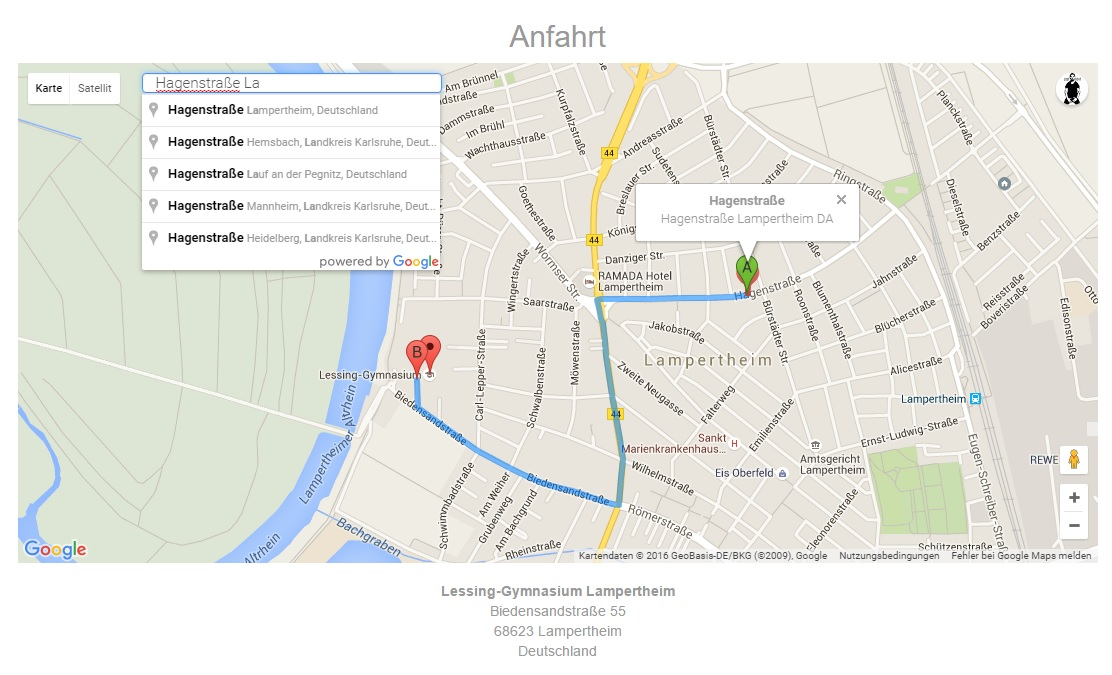
\includegraphics[scale=0.5]{img/googleMaps.jpg}}
	\caption{Anfahrtbeschreibung mit Google Maps}
	\label{fig:googleMaps}
\end{figure}

Auf dem Bild ist nicht nur der Standort der Schule vermerkt, sondern darüberhinaus kann der User über ein Eingabefeld links oben seine Abfahrtsadresse eingeben, sodass die optimale Route auf der Karte angezeigt wird. Des Weiteren wurde mit Hilfe der Autocomplete Funktion der Google Maps API eine automatische Vervollständigung der Adresse bei Eingabe in das Adressfeld implementiert, wie auf dem Screenshot zu sehen ist.
\par
Verwirklicht wurde die Einbindung, indem zuerst



\section{Einbindung von Social Buttons mittels des Heise Plugins}
\label{Einbindung von Social Buttons mittels des Heise Plugins}



\chapter{Client-Server-Kommunikation}
\label{Client-Server-Kommunikation}

\section{Anmeldefunktion per AJAX-Calls}
\label{Anmeldefunktion per AJAX-Calls}

\subsection{Bereitstellung eines REST-Service mit node.js}
\label{Bereitstellung eines REST-Service mit node.js}

\subsection{Konsumieren der Daten im Frontent mit AJAX-Calls}
\label{Konsumieren der Daten im Frontent mit AJAX-Calls}

%	Literaturverzeichnis 	
\ihead{} % Neue Header-Definition 
\printbibliography	

% Der Anhang beginnt hier - jedes Kapitel wird alphabetisch aufgezählt. (Anhang A, B usw.)
\appendix
\ihead{\appendixname~\thechapter} % Neue Header-Definition





% Ehrenwörtliche Erklärung
\clearpage
\chapter*{Ehrenwörtliche Erklärung}	

% Wird die folgende Zeile auskommentiert, erscheint die ehrenwörtliche 
% Erklärung im Inhaltsverzeichnis. 

% \addcontentsline{toc}{chapter}{Ehrenwörtliche Erklärung}  

Ich erkläre hiermit ehrenwörtlich: 

\begin{enumerate}
	\item dass ich die hier vorliegende Arbeit mit dem Thema \textit{Titel der Arbeit} ohne fremde Hilfe angefertigt habe; 
	\item dass ich die Übernahme wörtlicher Zitate aus der Literatur sowie die Verwendung der Gedanken anderer Autoren an den entsprechenden Stellen innerhalb der Bachelorarbeit gekennzeichnet habe;
	\item dass ich die vorliegende Arbeit bei keiner anderen Prüfung vorgelegt habe; 
	\item dass die eingereichte elektronische Fassung exakt mit der eingereichten schriftlichen Fassung übereinstimmt.
\end{enumerate}
Ich bin mir bewusst, dass eine falsche Erklärung rechtliche Folgen haben wird.

\vspace{3cm}
Ort, Datum \hfill Unterschrift 


\end{document}